\documentclass[xcolor=svgnames]{beamer}
\usetheme[
    %%% options passed to the outer theme
    %    hidetitle,           % hide the (short) title in the sidebar
    %    hideauthor,          % hide the (short) author in the sidebar
    %    hideinstitute,       % hide the (short) institute in the bottom of the sidebar
    %    shownavsym,          % show the navigation symbols
         width=1.5cm,         % width of the sidebar (default is 2 cm)
    %    hideothersubsections,% hide all subsections but the subsections in the current section
    %    hideallsubsections,  % hide all subsections
         left                 % right of left position of sidebar (default is right)
    %%% options passed to the color theme
        lightheaderbg         % use a light header background
  ]{AAUsidebar}

% #### graphics and schemes
\usepackage{graphicx}
\graphicspath{{img/}}
\usepackage{tikz}
\usetikzlibrary{                          % TikZ libraries
                scopes,                   % .
                shapes,                   % .
                arrows,                   % .
                through,                  % .
                calc,                     % .
                intersections,            % .
                spy,                      % .
                matrix,                   % .
                chains,                   % .
                decorations.pathreplacing,% .
                decorations.pathmorphing, % .
                decorations.markings}     % .

\usepackage{pgfplots}                     % TikZ plots
\usepackage{pgfplotstable}                % TikZ tables from CSV
\pgfplotsset{compat=1.3}                  % activates \xilabel shift` for pgfplots
\usepackage{array}
\usepackage{listings}
\usepackage{ccicons}
\usepackage{tcolorbox}
\usepackage{listings}                     % code
\usepackage{adjustbox}                    % code
\usepackage{eurosym}                      % euro symbol
\usepackage{attrib}

% #### colors
\usepackage{xcolor}                       % common color names
\usepackage{colortbl}                     % common color names

% #### layouts
\usepackage{multicol}
\usepackage[textfont=footnotesize,bf]{caption}
\usepackage{subfig}

% #### math
\usepackage{siunitx}

% #### fonts
\usepackage[utf8]{inputenc}
\usepackage[italian]{babel}
\usepackage[T1]{fontenc}
\usepackage{cmbright}
\usepackage{soul} %slanted text
\usepackage{hyperref}
\urlstyle{same}
\hypersetup{pdfauthor={Francesco de Virgilio},pdftitle={Geostatistica con GIS open source:\\gli insediamenti neolitici del Tavoliere}}

% #### tables
\usepackage{booktabs}			          % migliora la qualità delle tabelle
\usepackage{tabularx}			          % colonne a spaziatura fissa delle tabelle
\newcommand{\otoprule}                    % better top rule horizontal line
    {\midrule[\heavyrulewidth]}           % .

% #### mainmatter
\title[Geostatistica con GIS open source]{Geostatistica con GIS open source}
\subtitle{Gli insediamenti neolitici del Tavoliere\\{\tiny Tesi di laurea triennale in Geofisica applicata}}
\author[Francesco \mbox{de Virgilio}]{
    Francesco de Virgilio\\\vspace{0.05\textwidth}
    {\scriptsize
        Relatore: Ch.mo Prof. Marcello Ciminale\\
        ~~Correlatrice: dott.ssa Mariangela Noviello
    }
}
\date{}

% ### title page logo
\pgfdeclareimage[height=1.5cm]{titlepagelogo}{AAUgraphics/uniba} % placed on the title page
\titlegraphic{% is placed on the bottom of the title page
    \pgfuseimage{titlepagelogo}\\\vspace{-0.02\textwidth}
    {\tiny Dipartimento di Scienze della Terra e Geoambientali\\\vspace{-0.02\textwidth}
     Università degli Studi di Bari ``Aldo Moro''
    }
}

\begin{document}
    {\aauwavesbg%
        \begin{frame}[plain,noframenumbering]
            \titlepage
        \end{frame}
    }

    %\begin{frame}{Tirocinio}
        %\begin{columns}[c]
            %\column{0.48\textwidth}
            %\centering
            %\begin{figure}
                %\centering
                %\includegraphics[width=0.5\textwidth]{AAUgraphics/uniba}
            %\end{figure}
            %\vspace{-0.2\textwidth}
            %Dip. di Scienze della Terra e Geoambientali\\
            %Università di Bari ``Aldo Moro''
            %\column{0.48\textwidth}
            %\centering
            %\begin{figure}
                %\centering
                %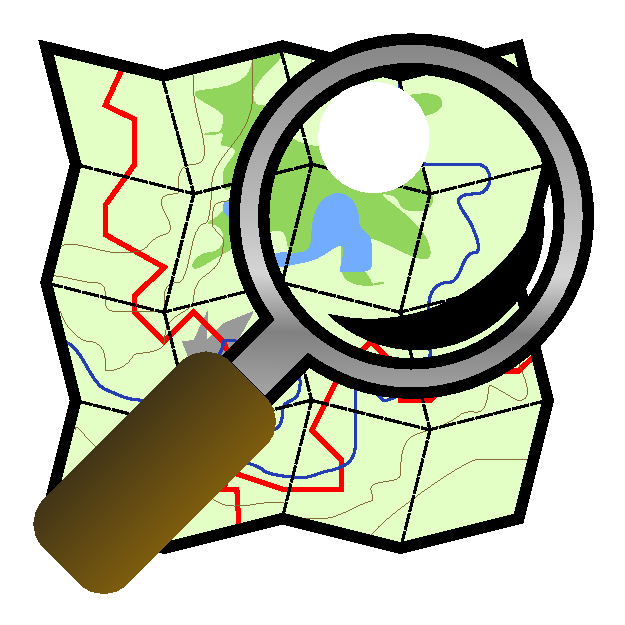
\includegraphics[width=0.5\textwidth]{img/logo}
            %\end{figure}
            %\vspace{-0.1\textwidth}
            %L.--P. Archaeology\\
            %Londra, Regno Unito
        %\end{columns}
    %\end{frame}

    \begin{frame}{Insediamenti neolitici}
        \centering
        \begin{tikzpicture}
            \node[anchor=south west,inner sep=0] at (0,0) {\includegraphics[width=\textwidth]{img/aerea}};
            \pause
            \draw [thick,draw=red,double] (7.1,4) -- (7.3,3.9) -- (7.5,3.84) -- (7.8,3.7) -- (8.1,3.5) -- (8.2,3.3) -- (7.9,2.5) -- (6.7,1.85) -- (5.5,1.5) -- (5,1.35) -- (4.5,1.3) -- (3.8,1.25) -- (3.4,1.3) -- (3,1.35) -- (2.8,1.38) -- (2.7,1.4) -- (2.4,1.5) -- (2,1.65) -- (1.8,1.8);
            \draw [thick,draw=red,double] (2.8,3.8) -- (3.2,3.9) -- (4.68,4.15) -- (4.7,4.05);
            \draw [thick,draw=red,double] (4.89,4.05) -- (4.85,4.18) -- (6,4.3);
            \node [thick,draw=blue!50,fill=black!10,rounded corners] (ditch-label) at (6.8,4.6) {\tiny{ditch}};
            \pause
            \node [draw,thick,dashed,circle,inner sep=9pt] (comp1) at (3.75,2.8) {};
            \node [draw,thick,dashed,circle,inner sep=9pt] (comp2) at (5.35,2.3) {};
            \node [draw,thick,dashed,circle,inner sep=9pt] (comp3) at (5.95,3.45) {};
            \node [thick,draw=blue!50,fill=black!10,rounded corners] (compound-label) at (6.7,2.6) {\tiny{compounds}};
            \draw [->] (compound-label.west) to [bend right=30] (comp1);
            \draw [->] (compound-label.south) to [bend left=30] (comp2);
            \draw [->] (compound-label.north) to [bend right=20] (comp3);
        \end{tikzpicture}
    \end{frame}

    \section{Workflow}
        \begin{frame}{Il workflow dell'analisi geofisica}
            \resizebox{1\textwidth}{!}{%
                \begin{tikzpicture}
                    \input{img/dot-flow-general}
                \end{tikzpicture}
            }
        \end{frame}

        \begin{frame}{Il workflow dell'analisi geofisica}
            \resizebox{1\textwidth}{!}{%
                \begin{tikzpicture}
                    \input{img/dot-flow-general-1}
                \end{tikzpicture}
            }
        \end{frame}

        \begin{frame}{Il workflow dell'analisi geofisica}
            \resizebox{1\textwidth}{!}{%
                \begin{tikzpicture}
                    \input{img/dot-flow-general-2}
                \end{tikzpicture}
            }
        \end{frame}

    \section{Compounds}
        \begin{frame}{Compounds: difficoltà e stato dell'arte}
            \begin{columns}[c]
                \column{0.5\textwidth}
                \centering
                \only<1>{
                    \includegraphics[width=0.8\textwidth]{img/niekamp}\\
                    A. Niekamp --- 2013\\
                    Pietrele, Romania
                }
                \column{0.5\textwidth}
            \end{columns}
        \end{frame}

        \begin{frame}{Compounds: difficoltà e stato dell'arte}
            \begin{columns}[c]
                \column{0.5\textwidth}
                    \centering
                    \begin{tikzpicture}
                        %\draw [help lines] (0,0) grid (4,3);
                        \draw [very thick,draw=blue!50,fill=black!20,rounded corners] (0,0) rectangle (1.5,2);
                        \draw[red,->] (0.75,-0.2) -- (0.75,2.5);
                    \end{tikzpicture}\\
                    A. Niekamp --- 2013\\
                    Pietrele, Romania
                \pause
                \column{0.5\textwidth}
                    \centering
                    \only<2-3>{
                        \begin{tikzpicture}[scale=0.007]
                            \input{img/comp-simple}
                            \begin{scope}[yshift=210em,xshift=150em,scale=0.90]
                                \input{img/comp-ang-area-simple}
                            \end{scope}
                        \end{tikzpicture}
                        \pause
                        \begin{tikzpicture}[remember picture,overlay]
                            \node (per) at (0.5,1) {\tiny perimetro};
                            \node (area) at (-1.7,-0.5) {\tiny area};
                            \node[align=center] (acc-up) at (-3,2.5) {\tiny orientazione};
                            \node[align=center] (acc) at (-3,2.2) {\tiny (accesso)};
                            \draw[draw=red,fill=red] (-2.15,1.38) circle (1pt) coordinate(acc-n);
                            \draw[draw=red,fill=red] (-2.08,0.6) circle (1pt) coordinate(acc-s);
                            \draw[draw=red,fill=red] (acc-n) -- (acc-s);
                            \draw[->,>=*] (acc.south) to [bend right=55] ($ (acc-n)!.5!(acc-s) $);
                            \draw[->,>=*] (area.north) to [bend right=10] (-1.2,1);
                            \draw[->,>=*] (per.south) to [bend left=65] (-0.8,0.5);
                        \end{tikzpicture}
                    }
                    \pause
                    \begin{tikzpicture}[overlay,scale=0.007,yshift=-224cm,xshift=-368cm]
                        \input{img/comp-simple}
                    \end{tikzpicture}
                    \begin{tikzpicture}[remember picture,overlay]
                        \node (label) at (-0.5,-1.22) {A. Laterza --- 2013};
                        \node (label) at (-0.5,-1.7) {Tavoliere, Puglia};
                    \end{tikzpicture}
            \end{columns}
        \end{frame}

    \section{Distinzione}
        \begin{frame}{Distinzione di \emph{ditches} e \emph{compounds}: Jenks}
            \small{Anglisano (Lucera): 47 geometrie}\\
            \centering
            \scalebox{1}[-1]{ % mirror image
                \begin{tikzpicture}[x=1mm,y=1mm,scale=0.15]
                    \input{img/jenks-bn}
                \end{tikzpicture}
            }\\
            \vspace{0.05\textwidth}
            Dati geografici di partenza\\
            ~
        \end{frame}

        \begin{frame}{Distinzione di \emph{ditches} e \emph{compounds}: Jenks}
            \small{Anglisano (Lucera): 47 geometrie}\\
            \centering
            \scalebox{1}[-1]{ % mirror image
                \begin{tikzpicture}[x=1mm,y=1mm,scale=0.15]
                    \input{img/jenks}
                \end{tikzpicture}
            }\\
            \vspace{0.05\textwidth}
            Classificazione dei \textbf{perimetri} con intervalli naturali di Jenks, $k=5$\\
            \small{
                \emph{ditches}: classi 1, 2\quad\quad\emph{compounds}: classi 3, 4, 5
            }
        \end{frame}

        \begin{frame}{Distinzione di \emph{ditches} e \emph{compounds}: Jenks}
            \small{Anglisano (Lucera): 47 geometrie = 3 ditches + 44 compounds}\\
            \centering
            \scalebox{1}[-1]{ % mirror image
                \begin{tikzpicture}[x=1mm,y=1mm,scale=0.15]
                    \input{img/jenks-2col}
                \end{tikzpicture}
            }\\
            \vspace{0.05\textwidth}
            \small{
                ~\\
                ~
            }\\
            \pause
            \begin{tikzpicture}[remember picture,overlay]
                \node (dit) at (0.2,1.5) {\scriptsize ditches};
                \draw[->,>=*] (dit.north) to (-0.8,2.2);
                \draw[->,>=*] (dit.north) to [bend left=25] (0.8,2.7);
                \node (com) at (4,6.2) {\scriptsize compounds};
                \draw[->,>=*] (com.north) to [bend right=25] (2.2,6.6);
                \draw[->,>=*] (com.south) to [bend left=25] (2.4,5.8);
            \end{tikzpicture}\\
        \end{frame}

    \section{Area, perim.}

        \begin{frame}{Derivazione aree e perimetro}
            \begin{columns}[c]
                \column{0.4\textwidth}
                \centering
                    \begin{description}
                        \item[$C$]\hfill\\ centroide
                        \item[$F$]\hfill\\ punto più distante da $C$
                        \item[$B$]\hfill\\ buffer da $F$
                    \end{description}
                \column{0.6\textwidth}
                \centering
                    \begin{tikzpicture}[x=2.5pt,y=2.5pt,scale=0.1
                            ]
                            \input{img/comp-iter-1} 
                    \end{tikzpicture}
            \end{columns}
        \end{frame}

        \begin{frame}{Derivazione aree e perimetro}
            \centering
            \begin{tikzpicture}[x=2.5pt,y=2.5pt,scale=0.1
                    ]
                \input{img/comp-iter-2} 
            \end{tikzpicture}
            \begin{tikzpicture}[remember picture,overlay]
                \node[rectangle, rounded corners, draw=blue!40, align=center] (xy) at (1,4.5) {
                    \scriptsize$\alpha=\SI{1}{\degree}$\\
                    \scriptsize$x_p=x_C + r\cdot\cos{\alpha}$\\
                    \scriptsize$y_p = y_C + r\cdot\cos{\alpha}$
                };
                \draw[draw=blue!40] (xy.south) to [bend left=30] (-1,3);
            \end{tikzpicture}
        \end{frame}

        \begin{frame}{Derivazione aree e perimetro}
            \centering
            \begin{tikzpicture}[x=2.5pt,y=2.5pt,scale=0.1
                    ]
                \input{img/comp-iter-3} 
            \end{tikzpicture}
            \begin{tikzpicture}[remember picture,overlay]
                \node (label-i) at (-2.5,-0.7) {$I = \{ i_1 (x_{i_1}, y_{i_1})\}$};
                \node[rectangle, rounded corners, draw=blue!40, align=center] (xy) at (-6.8,2) {
                    \scriptsize$d_{i_2 C}<d_{i_1 C}$
                };
            \end{tikzpicture}
        \end{frame}

        \begin{frame}{Derivazione aree e perimetro}
            \centering
            \begin{tikzpicture}[x=2.5pt,y=2.5pt,scale=0.1
                    ]
                \input{img/comp-iter-3-1} 
            \end{tikzpicture}
            \begin{tikzpicture}[remember picture,overlay]
                \node (label-i) at (-2.5,-0.7) {$I = \{ i_1 (x_{i_1}, y_{i_1}), i_2 (x_{i_2}, y_{i_2})\}$};
            \end{tikzpicture}
        \end{frame}

        \begin{frame}{Derivazione aree e perimetro}
            \centering
            \begin{tikzpicture}[x=2.5pt,y=2.5pt,scale=0.1
                    ]
                \input{img/comp-iter-3-2} 
            \end{tikzpicture}
            \begin{tikzpicture}[remember picture,overlay]
                \node (label-i) at (-2.5,-0.7) {$I = \{ i_1 (x_{i_1}, y_{i_1}), i_2 (x_{i_2}, y_{i_2}), i_3 (x_{i_3}, y_{i_3})\}$};
            \end{tikzpicture}
        \end{frame}

        \begin{frame}{Derivazione aree e perimetro}
            \centering
            \begin{tikzpicture}[x=2.5pt,y=2.5pt,scale=0.1
                    ]
                \input{img/comp-iter-3-3}
            \end{tikzpicture}
            \begin{tikzpicture}[remember picture,overlay]
                \node (label-i) at (-2.5,-0.7) {$I = \{ i_1 (x_{i_1}, y_{i_1}), i_2 (x_{i_2}, y_{i_2}), i_3 (x_{i_3}, y_{i_3}), i_4 (x_{i_4}, y_{i_4}), \ldots \}$};
            \end{tikzpicture}
        \end{frame}

        \begin{frame}{Derivazione aree e perimetro}
            \centering
            \begin{tikzpicture}[x=2.5pt,y=2.5pt,scale=0.1
                    ]
                \input{img/comp-iter-4} 
            \end{tikzpicture}
            \begin{tikzpicture}[remember picture,overlay]
                \node (label-i) at (-1.5,-1) {$I = \{ i_1 (x_{i_1}, y_{i_1}), i_2 (x_{i_2}, y_{i_2}), i_3 (x_{i_3}, y_{i_3}), i_4 (x_{i_4}, y_{i_4}), \ldots \}$};
            \end{tikzpicture}
        \end{frame}

        \begin{frame}{Derivazione aree e perimetro}
            \centering
            \begin{tikzpicture}[x=2.5pt,y=2.5pt,scale=0.1
                    ]
                \input{img/comp-iter-4} 
                \begin{scope}[yshift=27em,xshift=49em,scale=0.90]
                    \input{img/comp-ang-area-simple}
                \end{scope}
            \end{tikzpicture}
            \begin{tikzpicture}[remember picture,overlay]
                \node (label-i) at (-1.5,-1) {$I = \{ i_1 (x_{i_1}, y_{i_1}), i_2 (x_{i_2}, y_{i_2}), i_3 (x_{i_3}, y_{i_3}), i_4 (x_{i_4}, y_{i_4}), \ldots \}$};
            \end{tikzpicture}
        \end{frame}

    \section{Accesso}
        \begin{frame}{Derivazione dell'accesso}     %% step 1
            \footnotesize
            \centering
            \begin{quote}
                Segmento \textbf{rettilineo} più lungo tra quelli che compongono il perimetro.
            \end{quote}
            \vfill
            \begin{columns}[c]
                \column{0.5\textwidth}
                \centering
                \Large
                \begin{align*}
                    d&=0\\
                    d &< d_{p_3, p_4}\\
                    d &= d_{p_3, p_4}
                \end{align*}
                \column{0.5\textwidth}
                \centering
                \begin{tikzpicture}[x=2.5pt,y=2.5pt,scale=0.1
                        ]
                    \input{img/comp-ang-area-simple}
                \end{tikzpicture}
                \begin{tikzpicture}[remember picture,overlay]
                    \tikzset{dot-int/.style={
    circle,
    draw=red,
    fill=red,
    inner sep=0,
    minimum size=3pt
    }
}

\node[dot-int] (pt1) at (-2.45,1.65) {};
\node[dot-int] (pt2) at (-2.2,1.7) {};
\node[dot-int] (pt3) at (-2,2) {};
\node[dot-int] (pt4) at (-1.6,2.25) {};
\node[dot-int] (pt5) at (-1.2,2.35) {};
\node[dot-int] (pt6) at (-0.8,2.4) {};
\node[dot-int] (pt7) at (-0.5,2.2) {};
\node[dot-int] (pt8) at (-0.3,1.8) {};
\node[dot-int] (pt9) at (-0.15,1.4) {};
\node[dot-int] (pt10) at (-0.2,0.6) {};
\node[dot-int] (pt11) at (-0.4,0.3) {};
\node[dot-int] (pt12) at (-0.9,0.05) {};
\node[dot-int] (pt13) at (-1.6,0.05) {};
\node[dot-int] (pt14) at (-2.3,0.5) {};

                    \node[dot-int,pin=100:$p_3$] (pt3) at (-2,2) {};
                    \node[dot-int,pin=90:$p_4$] (pt4) at (-1.6,2.25) {};
                    \draw[very thick,draw=blue] (pt3) -- (pt4);
                \end{tikzpicture}
            \end{columns}
        \end{frame}

        \begin{frame}{Derivazione dell'accesso}     %% step 2
            \footnotesize
            \centering
            \begin{quote}
                Segmento \textbf{rettilineo} più lungo tra quelli che compongono il perimetro.
            \end{quote}
            \vfill
            \begin{columns}[c]
                \column{0.5\textwidth}
                \centering
                \Large
                \begin{align*}
                    d &= d_{p_3, p_4}\\
                    d &> d_{p_6, p_7}\\
                    d &= d_{p_3, p_4}
                \end{align*}
                \column{0.5\textwidth}
                \centering
                \begin{tikzpicture}[x=2.5pt,y=2.5pt,scale=0.1
                        ]
                    \input{img/comp-ang-area-simple}
                \end{tikzpicture}
                \begin{tikzpicture}[remember picture,overlay]
                    \tikzset{dot-int/.style={
    circle,
    draw=red,
    fill=red,
    inner sep=0,
    minimum size=3pt
    }
}

\node[dot-int] (pt1) at (-2.45,1.65) {};
\node[dot-int] (pt2) at (-2.2,1.7) {};
\node[dot-int] (pt3) at (-2,2) {};
\node[dot-int] (pt4) at (-1.6,2.25) {};
\node[dot-int] (pt5) at (-1.2,2.35) {};
\node[dot-int] (pt6) at (-0.8,2.4) {};
\node[dot-int] (pt7) at (-0.5,2.2) {};
\node[dot-int] (pt8) at (-0.3,1.8) {};
\node[dot-int] (pt9) at (-0.15,1.4) {};
\node[dot-int] (pt10) at (-0.2,0.6) {};
\node[dot-int] (pt11) at (-0.4,0.3) {};
\node[dot-int] (pt12) at (-0.9,0.05) {};
\node[dot-int] (pt13) at (-1.6,0.05) {};
\node[dot-int] (pt14) at (-2.3,0.5) {};

                    \node[dot-int,pin=90:$p_6$] (pt6) at (-0.8,2.4) {};
                    \node[dot-int,pin=70:$p_7$] (pt7) at (-0.5,2.2) {};
                    \draw[very thick,draw=blue] (pt6) -- (pt7);
                \end{tikzpicture}
            \end{columns}
        \end{frame}

        \begin{frame}{Derivazione dell'accesso}     %% step 3
            \footnotesize
            \centering
            \begin{quote}
                Segmento \textbf{rettilineo} più lungo tra quelli che compongono il perimetro.
            \end{quote}
            \vfill
            \begin{columns}[c]
                \column{0.5\textwidth}
                \centering
                \Large
                \begin{align*}
                    d &= d_{p_3, p_4}\\
                    d &< d_{p_9, p_{10}}\\
                    d &= d_{p_9, p_{10}}
                \end{align*}
                \column{0.5\textwidth}
                \centering
                \begin{tikzpicture}[x=2.5pt,y=2.5pt,scale=0.1
                        ]
                    \input{img/comp-ang-area-simple}
                \end{tikzpicture}
                \begin{tikzpicture}[remember picture,overlay]
                    \tikzset{dot-int/.style={
    circle,
    draw=red,
    fill=red,
    inner sep=0,
    minimum size=3pt
    }
}

\node[dot-int] (pt1) at (-2.45,1.65) {};
\node[dot-int] (pt2) at (-2.2,1.7) {};
\node[dot-int] (pt3) at (-2,2) {};
\node[dot-int] (pt4) at (-1.6,2.25) {};
\node[dot-int] (pt5) at (-1.2,2.35) {};
\node[dot-int] (pt6) at (-0.8,2.4) {};
\node[dot-int] (pt7) at (-0.5,2.2) {};
\node[dot-int] (pt8) at (-0.3,1.8) {};
\node[dot-int] (pt9) at (-0.15,1.4) {};
\node[dot-int] (pt10) at (-0.2,0.6) {};
\node[dot-int] (pt11) at (-0.4,0.3) {};
\node[dot-int] (pt12) at (-0.9,0.05) {};
\node[dot-int] (pt13) at (-1.6,0.05) {};
\node[dot-int] (pt14) at (-2.3,0.5) {};

                    \node[dot-int,pin=10:$p_9$] (pt9) at (-0.15,1.4) {};
                    \node[dot-int,pin=-10:$p_{10}$] (pt10) at (-0.2,0.6) {};
                    \draw[very thick,draw=blue] (pt9) -- (pt10);
                \end{tikzpicture}
            \end{columns}
        \end{frame}

        \begin{frame}{Derivazione dell'accesso}     %% step 4
            \footnotesize
            \centering
            \begin{quote}
                Segmento \textbf{rettilineo} più lungo tra quelli che compongono il perimetro.
            \end{quote}
            \vfill
            \begin{columns}[c]
                \column{0.5\textwidth}
                \centering
                \Large
                \begin{align*}
                    d &= d_{p_9, p_{10}}\\
                    d &> d_{p_{12}, p_{13}}\\
                    d &= d_{p_9, p_{10}}
                \end{align*}
                \column{0.5\textwidth}
                \centering
                \begin{tikzpicture}[x=2.5pt,y=2.5pt,scale=0.1
                        ]
                    \input{img/comp-ang-area-simple}
                \end{tikzpicture}
                \begin{tikzpicture}[remember picture,overlay]
                    \tikzset{dot-int/.style={
    circle,
    draw=red,
    fill=red,
    inner sep=0,
    minimum size=3pt
    }
}

\node[dot-int] (pt1) at (-2.45,1.65) {};
\node[dot-int] (pt2) at (-2.2,1.7) {};
\node[dot-int] (pt3) at (-2,2) {};
\node[dot-int] (pt4) at (-1.6,2.25) {};
\node[dot-int] (pt5) at (-1.2,2.35) {};
\node[dot-int] (pt6) at (-0.8,2.4) {};
\node[dot-int] (pt7) at (-0.5,2.2) {};
\node[dot-int] (pt8) at (-0.3,1.8) {};
\node[dot-int] (pt9) at (-0.15,1.4) {};
\node[dot-int] (pt10) at (-0.2,0.6) {};
\node[dot-int] (pt11) at (-0.4,0.3) {};
\node[dot-int] (pt12) at (-0.9,0.05) {};
\node[dot-int] (pt13) at (-1.6,0.05) {};
\node[dot-int] (pt14) at (-2.3,0.5) {};

                    \node[dot-int,pin=-80:$p_{12}$] (pt12) at (-0.9,0.05) {};
                    \node[dot-int,pin=-100:$p_{13}$] (pt13) at (-1.6,0.05) {};
                    \draw[very thick,draw=blue] (pt12) -- (pt13);
                \end{tikzpicture}
            \end{columns}
        \end{frame}

        \begin{frame}{Derivazione dell'accesso}     % step 5
            \footnotesize
            \centering
            \begin{quote}
                Segmento \textbf{rettilineo} più lungo tra quelli che compongono il perimetro.
            \end{quote}
            \vfill
            \begin{columns}[c]
                \column{0.5\textwidth}
                \centering
                \Large
                \begin{align*}
                    d &= d_{p_9, p_{10}}\\
                    d &< d_{p_{14}, p_{1}}\\
                    d &= d_{p_{14}, p_{1}}
                \end{align*}
                \column{0.5\textwidth}
                \centering
                \begin{tikzpicture}[x=2.5pt,y=2.5pt,scale=0.1
                        ]
                    \input{img/comp-ang-area-simple}
                \end{tikzpicture}
                \begin{tikzpicture}[remember picture,overlay]
                    \tikzset{dot-int/.style={
    circle,
    draw=red,
    fill=red,
    inner sep=0,
    minimum size=3pt
    }
}

\node[dot-int] (pt1) at (-2.45,1.65) {};
\node[dot-int] (pt2) at (-2.2,1.7) {};
\node[dot-int] (pt3) at (-2,2) {};
\node[dot-int] (pt4) at (-1.6,2.25) {};
\node[dot-int] (pt5) at (-1.2,2.35) {};
\node[dot-int] (pt6) at (-0.8,2.4) {};
\node[dot-int] (pt7) at (-0.5,2.2) {};
\node[dot-int] (pt8) at (-0.3,1.8) {};
\node[dot-int] (pt9) at (-0.15,1.4) {};
\node[dot-int] (pt10) at (-0.2,0.6) {};
\node[dot-int] (pt11) at (-0.4,0.3) {};
\node[dot-int] (pt12) at (-0.9,0.05) {};
\node[dot-int] (pt13) at (-1.6,0.05) {};
\node[dot-int] (pt14) at (-2.3,0.5) {};

                    \node[dot-int,pin=120:$p_{1}$] (pt1) at (-2.45,1.65) {};
                    \node[dot-int,pin=-120:$p_{14}$] (pt14) at (-2.3,0.5) {};
                    \draw[very thick,draw=green] (pt14) -- (pt1);
                \end{tikzpicture}
            \end{columns}
        \end{frame}

        \begin{frame}{Derivazione dell'accesso}     %% final
            \footnotesize
            \centering
            \begin{columns}[c]
                \column{0.5\textwidth}
                \centering
                    \resizebox{1\textwidth}{!}{%
                        \input{img/dot-flow-access}
                    }
                \column{0.5\textwidth}
                \centering
                \begin{tikzpicture}[x=2.5pt,y=2.5pt,scale=0.1
                        ]
                    \input{img/comp-ang-area-simple}
                \end{tikzpicture}
                \begin{tikzpicture}[remember picture,overlay]
                    \tikzset{dot-int/.style={
    circle,
    draw=red,
    fill=red,
    inner sep=0,
    minimum size=3pt
    }
}

\node[dot-int] (pt1) at (-2.45,1.65) {};
\node[dot-int] (pt2) at (-2.2,1.7) {};
\node[dot-int] (pt3) at (-2,2) {};
\node[dot-int] (pt4) at (-1.6,2.25) {};
\node[dot-int] (pt5) at (-1.2,2.35) {};
\node[dot-int] (pt6) at (-0.8,2.4) {};
\node[dot-int] (pt7) at (-0.5,2.2) {};
\node[dot-int] (pt8) at (-0.3,1.8) {};
\node[dot-int] (pt9) at (-0.15,1.4) {};
\node[dot-int] (pt10) at (-0.2,0.6) {};
\node[dot-int] (pt11) at (-0.4,0.3) {};
\node[dot-int] (pt12) at (-0.9,0.05) {};
\node[dot-int] (pt13) at (-1.6,0.05) {};
\node[dot-int] (pt14) at (-2.3,0.5) {};

                    \draw[very thick,draw=green] (pt14) -- (pt1);
                \end{tikzpicture}
            \end{columns}
        \end{frame}

    \section{Orientazione}

        \begin{frame}{Calcolo dell'orientazione}
            \centering
            \begin{tikzpicture}[x=2.5pt,y=2.5pt,scale=0.1
                    ]
                    \input{img/comp-orient-1}
            \end{tikzpicture}
            \begin{tikzpicture}[remember picture,overlay]
                \node[rectangle, rounded corners, draw=blue!40, align=center] (e-point) at (-4,3.5) {
                    \scriptsize$(x_e, y_e) = (\frac{1}{2}\left(x_1 + x_2\right),\frac{1}{2}\left(y_1 + y_2\right))$
                };
                \draw[->,draw=blue!40] (e-point.south) to [bend right=30] (-2.7,1.4);
            \end{tikzpicture}
        \end{frame}

        \begin{frame}{Calcolo dell'orientazione}
            \centering
            \begin{tikzpicture}[x=2.5pt,y=2.5pt,scale=0.1
                    ]
                    \input{img/comp-orient-2}
            \end{tikzpicture}
            \begin{tikzpicture}[remember picture,overlay]
                \node[rectangle, rounded corners, draw=blue!40, align=center] (card-label) at (1,4.5) {
                    \scriptsize$\alpha=\SI{45}{\degree}$\\
                    \scriptsize$x_p=x_C + r\cdot\cos{\alpha}$\\
                    \scriptsize$y_p = y_C + r\cdot\cos{\alpha}$
                };
                \draw[draw=blue!40] (card-label.south) to [bend left=30] (-0.5,3.1);
            \end{tikzpicture}
        \end{frame}

        \begin{frame}{Calcolo dell'orientazione}
            \centering
            \begin{tikzpicture}[x=2.5pt,y=2.5pt,scale=0.1
                    ]
                    \input{img/comp-orient-2-1}
            \end{tikzpicture}
        \end{frame}

    \lstset{
        language=python,
        numbers=left,
        numberstyle=\tiny,
        showstringspaces=false,
        aboveskip=-40pt,
        frame=leftline,
        basicstyle=\tiny
    }

    \section{Codice}

        \begin{frame}[fragile]
        \frametitle{Dalla logica al codice}     %% final with code
            \begin{columns}[c]
                \column{0.5\textwidth}
                \centering
                    \resizebox{1\textwidth}{!}{%
                        \input{img/dot-flow-access}
                    }
                \column{0.5\textwidth}
                \begin{adjustbox}{width=0.9\textwidth,keepaspectratio}
                    \begin{lstlisting}
# iterate on all open compounds
for compound in cur_shp.helpercompoundsarea_set \
        .filter(type='compound', open=True):
    # get sides and relative lengths as dictionary
    sides = get_side_dict(compound, 3857)
    # get longest side in area polygon as a LineString
    access_linestr = max(sides, key=sides.get)

    # get access lenght as projected value
    proj_access_linestr = access_linestr
    proj_access_linestr.transform(cur_shp.proj)

    # get the centroid of the access side
    feature_centroid = compound.poly.centroid

    # get compound's farthest point from centroid
    max_point = Point(compound.poly.convex_hull.extent[2],
                      compound.poly.convex_hull.extent[3],
                      srid=3857)
    radius = max_point.distance(feature_centroid)

    # draw cardinal points around the compound every 
    # 45 degree, and rotate them by 12 degree 
    # to align perpendicularly to N
    cardinal_pts = get_round_vertex(
        45,
        radius,
        feature_centroid.x,
        feature_centroid.y,
        3857,
        12)

    # create "cake slices" using cardinal points
    polygon_list = []
    for i, item in enumerate(cardinal_pts):
        points = (feature_centroid.coords,
                  item.coords,
                  cardinal_pts[i - 1].coords,
                  feature_centroid.coords)
        polygon_list.append(Polygon(points, srid=3857))
    sectors = MultiPolygon(polygon_list, srid=3857)

    # get access side centroid
    access_centroid = access_linestr.centroid
    access_centroid.transform(3857)
                    \end{lstlisting}
                \end{adjustbox}
            \end{columns}
            % the following row must _not_ be indented: LaTeX will give you an error!
\end{frame} 

    \section{WebGIS}

        \begin{frame}{Interfaccia alle funzioni: webGIS}
            \includegraphics[width=1\textwidth]{img/shp-list}
        \end{frame}

        \begin{frame}{Interfaccia alle funzioni: webGIS}
            \includegraphics[width=1\textwidth]{img/shp-detail-1}
        \end{frame}

        \begin{frame}{Interfaccia alle funzioni: webGIS}
            \includegraphics[width=1\textwidth]{img/shp-wizard}
        \end{frame}

        \begin{frame}{Interfaccia alle funzioni: webGIS}
            \includegraphics[width=1\textwidth]{img/shp-detail-2}
        \end{frame}

        \begin{frame}{Interfaccia alle funzioni: webGIS}
            \includegraphics[width=1\textwidth]{img/shp-detail-3}
        \end{frame}

        \begin{frame}{Interfaccia alle funzioni: webGIS}
            \includegraphics[width=1\textwidth]{img/shp-detail-4}
        \end{frame}

        \begin{frame}{Interfaccia alle funzioni: webGIS}
            \includegraphics[width=1\textwidth]{img/shp-detail-5}
        \end{frame}

    \section{Statistiche}

        \begin{frame}{Affidabilità: numero di \emph{ditches} e \emph{compounds}}
            \centering
            \begin{tikzpicture}
                \input{tab/graph-num-compound}
            \end{tikzpicture}

            \begin{tikzpicture}
                \pgfplotstableread{tab/raw/number-ditch}{\loadedtable}
\small

\begin{axis}[
    width=1\textwidth,
    height=0.4\textwidth,
    bar width=5pt,
    ybar,
    ymin=0,
    enlarge x limits,
    xlabel=\tiny{insediamenti},
    xlabel shift=-5pt,
    ylabel=\scriptsize{ditches $(n)$},
    xtick={1,...,11},   % indicates xticks going from 1 to 11
    xticklabels from table={\loadedtable}{set},
    xticklabel style={rotate=45,font=\tiny},
    xticklabel shift=-3pt,
    yticklabel style={font=\tiny},
]
    \addplot table[x=id, y=laterza] from \loadedtable;
    \addplot table[x=id, y=current] from \loadedtable;
\end{axis}

            \end{tikzpicture}
        \end{frame}

        \begin{frame}{Affidabilità: aree e perimetri}
            \centering
            \begin{tikzpicture}
                \pgfplotstableread[col sep=comma]{tab/raw/aree.csv}{\loadedtable}
\small

\begin{axis}[
    width=1\textwidth,
    height=0.4\textwidth,
    bar width=5pt,
    ybar,
    ymin=0,
    enlarge x limits,
    ylabel=\scriptsize{area $(\si{\meter\squared})$},
    xtick={1,...,11},   % indicates xticks going from 1 to 11
    xticklabels from table={\loadedtable}{set},
    xticklabel style={rotate=45,font=\tiny},
    xticklabel shift=-3pt,
    yticklabel style={font=\tiny},
    legend style={font=\tiny,draw=black!40}
]
    \addplot table[x=id, y=laterza] from \loadedtable;
    \addplot table[x=id, y=current] from \loadedtable;
    \legend{Lat13,current}
\end{axis}

            \end{tikzpicture}

            \begin{tikzpicture}
                \input{tab/graph-perim}
            \end{tikzpicture}
        \end{frame}

        \begin{frame}{Affidabilità: aree e perimetri}
            \begin{tikzpicture}
                \pgfplotstableread[col sep=comma]{tab/raw/orient.csv}{\loadedtable}
\small

\begin{axis}[
    width=1\textwidth,
    height=0.45\textwidth,
    bar width=5pt,
    ybar,
    ymin=0,
    enlarge x limits,
    xlabel=\tiny{orientazione dei compounds},
    xlabel shift=-5pt,
    ylabel=\scriptsize{frequenza $(n)$},
    xtick={1,...,8},   % indicates xticks going from 1 to 11
    xticklabels from table={\loadedtable}{orient},
    xticklabel style={rotate=45,font=\tiny},
    xticklabel shift=-3pt,
    yticklabel style={font=\tiny},
    legend style={font=\tiny,legend pos=north west,draw=black!40}
]
    \addplot table[x=id, y=laterza] from \loadedtable;
    \addplot table[x=id, y=current] from \loadedtable;
    \legend{Lat13,current}
\end{axis}

            \end{tikzpicture}
            \pause
            \scriptsize
            \begin{align*}
                H_0 : \sigma^2_1 = \sigma^2_2   &&  s^2 &= \frac{1}{N-1} \sum_{i=1}^N (x_i - \overline{x})^2    &&  F_{\text{cal}} = \frac{s^2_2}{s^2_1} = 1.07\\
                H_a : \sigma^2_1\neq\sigma^2_2  &&  s^2_{1} &= 438.79   &&  F_{\text{cal}} < F_{\text{tab}}\\
                                                &&  s^2_{2} &= 470.84   &&  H_0\text{~verificata}
            \end{align*}
        \end{frame}

    \section{Conclusioni}

        \begin{frame}{Conclusioni}
            \centering
            Dati: 11 insediamenti -- 155 compounds
            \vfill
            \begin{tabular}[c]{ccc}
                \toprule
                &   Metodo standard     &   Metodo proposto\\
                \otoprule
                tempi           &   $\sim2$ mesi            &   $\sim\SI{30}{\minute}$\\\pause
                affidabilità    &   $100\%$                 &   $100\%$\\\pause
                riproducibilità &   parziale                &   completa\\\pause
                software        &   installazione locale    &   internet (webGIS)\\\pause
                costi           &   licenza GIS (\EUR{2850})&   open source: \EUR{0}\\
                \bottomrule
            \end{tabular}
        \end{frame}

        \begin{frame}
            \vfill
            \centering
            \Huge
            Grazie
            \vfill
            \scriptsize
            \begin{quote}
                \centering
                So Long, and Thanks for All the Fish\\
                \attrib{D. Adams}
            \end{quote}
            \vfill
        \end{frame}

\end{document}
